% This is samplepaper.tex, a sample chapter demonstrating the
% LLNCS macro package for Springer Computer Science proceedings;
% Version 2.21 of 2022/01/12
%
\documentclass[runningheads]{llncs}
\usepackage{esvect}
\usepackage[T1]{fontenc}
% T1 fonts will be used to generate the final print and online PDFs,
% so please use T1 fonts in your manuscript whenever possible.
% Other font encondings may result in incorrect characters.
%
\usepackage{graphicx}
% Used for displaying a sample figure. If possible, figure files should
% be included in EPS format.
%
% If you use the hyperref package, please uncomment the following two lines
% to display URLs in blue roman font according to Springer's eBook style:
%\usepackage{color}
%\renewcommand\UrlFont{\color{blue}\rmfamily}
%\urlstyle{rm}
%
\usepackage{amsfonts}
\usepackage{amsmath}
\usepackage{hyperref}
\usepackage{doi}
\usepackage{subcaption}
\usepackage[export]{adjustbox}
\usepackage{tabularx}
\usepackage{makecell}

\begin{document}
%
\title{Heuristic-Boosted Ejection Fraction Estimation from 2D U-Net Segmentation}
\titlerunning{Heuristic-Boosted EF Estimation}
%
%\titlerunning{Abbreviated paper title}
% If the paper title is too long for the running head, you can set
% an abbreviated paper title here
%
\author{Ernesto David Serize Portela\inst{1}\orcidID{0009-0009-4527-9977} \and
Amalia Rodríguez Sánchez\inst{1}\thanks{Corresponding author: amrsanchez@uclv.cu}\orcidID{0009-0007-3923-7442}  \and
José Carlos Serize Portela\inst{2}\orcidID{0009-0007-7979-7006} \and
MsC. Alejandro Cespón Ferriol\inst{1}\orcidID{0000-0002-8584-6958} \and
Dr. José Ignacio Ramírez Gómez\inst{3}\orcidID{0000-0003-3630-5722}}
\authorrunning{E.D. Serize, A. Rodríguez, J.C. Serize, MsC. A. Cespón, Dr. J.I. Ramírez}


\institute{
Universidad Central "Marta Abreu" de Las Villas, Santa Clara, Cuba\\
\url{http://www.uclv.edu.cu} \and
Constructor University, Bremen, Germany\\
\url{https://www.constructor.university} \and
Hospital Cardiocentro "Ernesto Che Guevara", Santa Clara, Cuba \\
}
%
\maketitle              % typeset the header of the contribution
%
\begin{abstract}

Ejection fraction (EF) estimation from apical four-chamber (A4C) echocardiogram videos is achieved through a pipeline combining deep learning segmentation and detailed analysis of ventricular geometry. A ResNet50-encoded 2D U-Net performs frame-by-frame left ventricle (LV) segmentation, with ventricular volumes subsequently calculated via the area-length method. To correct systematic biases arising from segmentation errors and heuristic volume estimation, the pipeline incorporates a regression model that predicts the signed error between ground truth and estimated EFs using a set of domain-informed features. The most informative predictors include the ventricular length ratio, volume ratio, and the variability in segmentation consistency over time, quantified as the standard deviation of the Dice similarity coefficient between consecutive frames. This approach achieves a mean absolute error (MAE) of 4.69\% on the EchoNet-Pediatric dataset for A4C views, offering an interpretable and refined estimation of cardiac function. 


\keywords{Ejection Fraction Estimation\and Cardiac Segmentation \and U-Net \and Echocardiography \and Pediatric Cardiology \and Area-Length Method \and Regression-Based Correction \and
Heart Failure Classification}

\end{abstract}

\section{Introduction}

Accurate estimation of ejection fraction plays a key role in assessing cardiac function. Traditionally, EF assessment relies on manual interpretation of echocardiogram videos, a process that is both time-consuming and prone to variability due to its subjective nature. This has driven a growing interest in automated methods that can provide fast, consistent, and objective measurements.

In recent years, this field has seen significant advances fueled by deep learning. LV segmentation has been addressed in several studies, many of which focus on 2D segmentation. Numerous efforts have improved U-Net architectures by incorporating attention mechanisms and residual connections \cite{azarmehr2020automated}\cite{moradi2019mfp}, while GAN-based data augmentation has helped address limited annotations \cite{kumar2025enhancing}. Lightweight U-Net and ResUnet variants have been effective for MRI segmentation \cite{irshad2023lightunet}\cite{xu2022resunet}, and adversarial learning combined with multi-stage pose estimation networks has enhanced the anatomical consistency of segmentation outputs\cite{wu2021automated}. Recently, hybrid models that combine convolutional neural networks (CNNs) with Transformer architectures have demonstrated promising results by capturing both fine-grained local details and broader global context in echocardiographic images \cite{shi2024study}. The publication of EchoNet-Dynamic\cite{ouyang2020echonet} introduced a video-based deep learning algorithm that achieves state-of-the-art performance and released a large public dataset of 10,030 annotated echocardiogram videos.

3D CNNs have shown high performance \cite{Ali2025}. However, their computational demands and limited interpretability pose significant implementations challenges, especially in low-resource environments. 

\begin{figure}
    \centering
    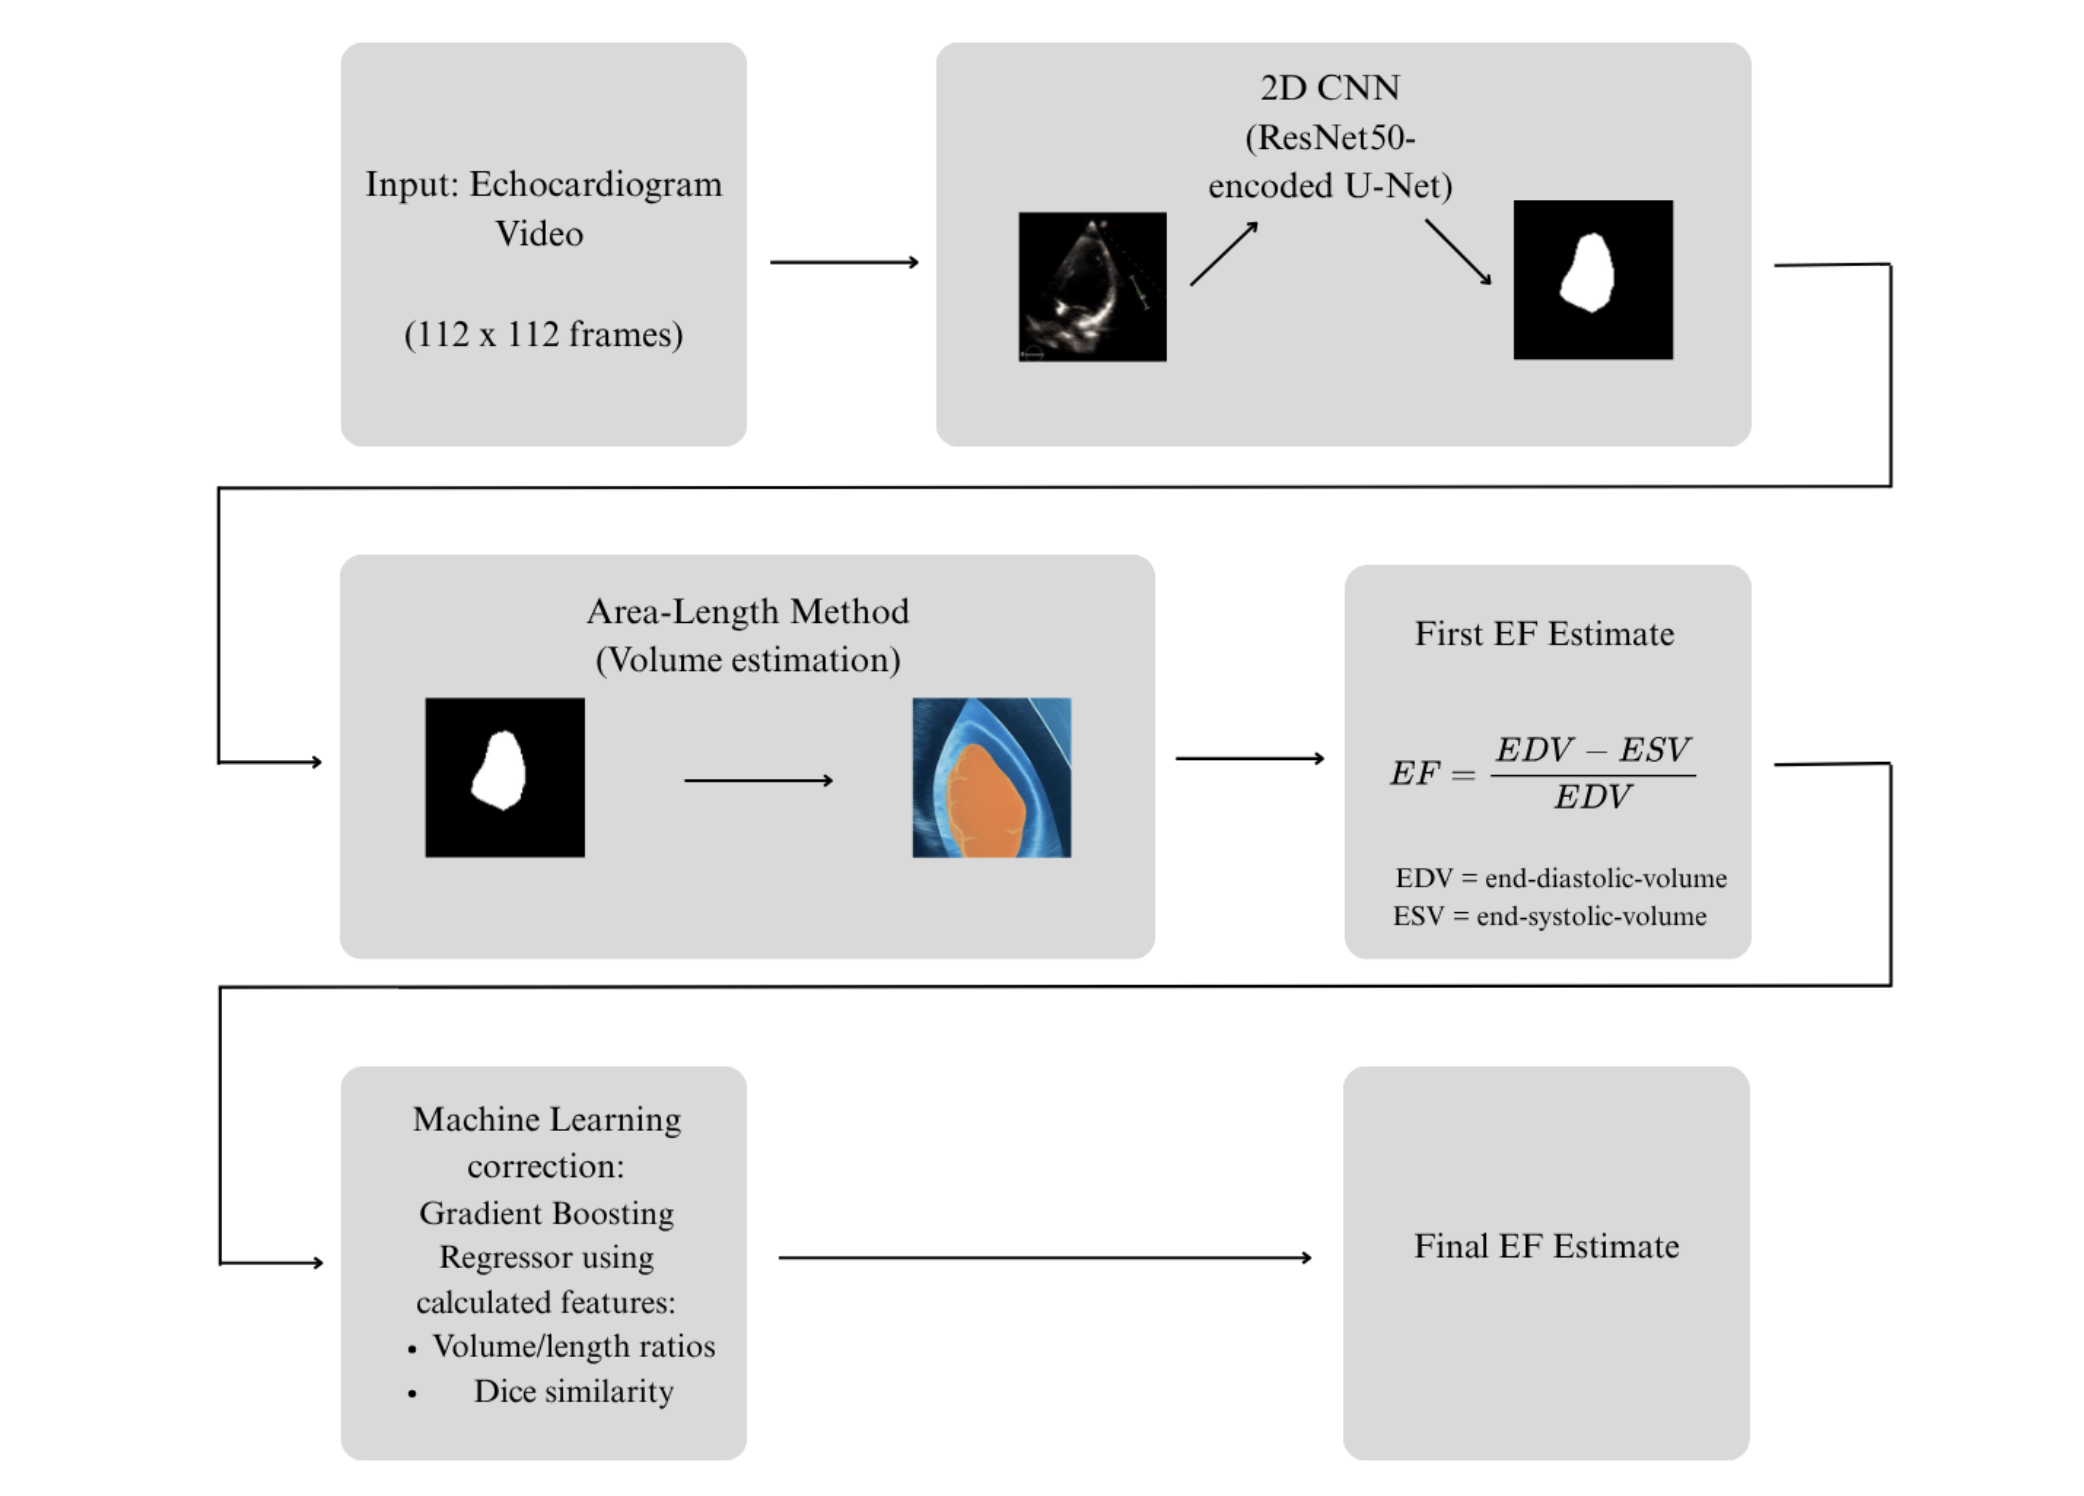
\includegraphics[width=0.8\linewidth]{diagram.png}
    \caption{Workflow diagram of the proposed ejection fraction estimation framework.}
    \label{fig:workflow-diagram}
\end{figure}

To address these challenges, frame-wise LV segmentation from A4C echocardiogram views is performed using a 2D U-Net with a ResNet50 encoder backbone (see Fig.\ref{fig:workflow-diagram}). Ventricular volumes and EF are subsequently estimated using the well-established area-length method, which is grounded in cardiac geometry\cite{Lang2015}.

Recognizing the inherent inaccuracies associated with this approach, a second stage was introduced: a regression model that estimates the signed error between true and predicted EF values. This model utilizes three input features: two geometric measures: the ventricular length ratio and the volume ratio, and a temporal consistency metric, defined as the standard deviation of the Dice similarity coefficient between consecutive segmentation outputs. The inclusion of this module not only significantly improves accuracy, but also offers an interpretable alternative to black-box deep learning models by leveraging features grounded in clinical relevance.

Building on this foundation, comprehensive statistical tests were conducted to confirm that the accuracy of the pipeline aligns with the standards of medical practice. An explainability analysis was also performed to clarify the factors that influence the model predictions. Together, these evaluations demonstrate technical rigor and practical reliability, aligning the pipeline as closely as possible with the needs and expectations of medical professionals.

\section{Materials and Methods}

\subsection{Dataset}
This investigation uses the A4C subset from EchoNet-Pediatric data\cite{echonetpediatric2023}, developed and published by researchers at Stanford University. It comprises 3,284 A4C video clips of pediatric patients aged from 0 to 18 years with a balanced gender distribution. Each video of $112\times112$ pixels consists of at least one cardiac cycle and includes expert manual LV tracings at end systole and end diastole. The data covers a wide range of cardiac function, with EF values ranging from 7. 02\% to 72. 99\%, reflecting various clinical conditions.

To train the segmentation model, an image-mask dataset was built by extracting and pairing two frames from each video, end-systole and end-diastole, with their associated binary segmentation masks, following the annotations and traced lines provided by Stanford. The samples were then divided into training, validation, and test sets, keeping the same video labels, ensuring methodological integrity.

\subsection{2D U-Net}

Among all deep learning approaches for medical image segmentation, encoder-decoder architectures have notable performance. The CAMUS project demonstrated that such models can accurately segment cardiac chambers and estimate clinical indices and significantly outperformed traditional methods in echocardiographic analysis \cite{leclerc2019camus}.

Based on these findings, to perform frame-by-frame segmentation, two 2D network architectures were implemented using PyTorch \cite{paszke2019pytorch}\cite{qubvel2019smp}: a standard U-Net and, to enhance this baseline, a U-Net with a ResNet50 encoder already pretrained on ImageNet\cite{deng2009imagenet}, with the goal of exploring whether transfer learning could improve segmentation accuracy. 

Both models were set up with similar conditions and trained, validated and tested in the same environment, using the previously described frame-mask dataset with the same data augmentation strategies—random rotations and horizontal flips—. The models operate on a normalized grayscale input image, and outputs a probability map.

A combination of binary cross-entropy and Dice loss was used, as is common in segmentation tasks, to balance pixel-wise accuracy with region-level overlap. Under this setup, both models showed stable convergence over the course of 20 training epochs. ResNet50-encoded U-Net outperformed the standard U-Net on the test set (see Table~\ref{tab:segmentation-comparison}), achieving higher mean and lower variability for Dice similarity and intersection-over-union (IoU) scores. 

\begin{table}[ht]
\centering
\caption{Comparison between Standard U-Net and ResNet50-encoded U-Net performance on the test set.}
\label{tab:segmentation-comparison}
\begin{tabular}{|l|c|c|}
\hline
\textbf{Metric} & \textbf{Standard U-Net} & \textbf{ResNet50-encoded U-Net} \\
\hline
Dice            & $0.903  (\pm 0.027$)       & $0.917  (\pm 0.02$ )              \\
IoU             & $0.824  (\pm 0.044$)       & $0.847  (\pm 0.034$)               \\
\hline
\end{tabular}
\end{table}

A hyperparameter optimization process was performed using Optuna\cite{akiba2019optuna} to improve segmentation performance. The best configuration found used a learning rate of 1e-4, batch size of 8, 20 training epochs and Adam optimizer for Resnet50-encoded U-Net.

\subsection{Ejection Fraction Estimation via Heuristic Area–Length Method}

For an echocardiogram video, each frame at time $t$ is passed as input to the segmentation model and the probability map outputted is thresholded by 0.5, to yield a binary mask $I_t \in \left\{0, 1\right\}$ (see Fig.\ref{fig:seg-sequence}), defining the region of interest as, 

\begin{equation}
\Omega_t\ =\ \left\{(x,y)\ \middle|{\ I}_t(x,y)\ =\ 1\right\}
\end{equation}

\begin{figure}
    \centering
    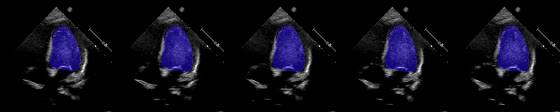
\includegraphics[width=0.9\linewidth]{segmentation_sequence.png}
    \caption{LV segmentation sequence across consecutive frames.}
    \label{fig:seg-sequence}
\end{figure}

Two key anatomical descriptors are computed from this mask: the area $\left|\Omega_t\right|$, defined as the total number of pixels within the segmented ventricle, and the length $L_t$,


\begin{equation}
L_t = \max_{(x_i, y_i),\, (x_j, y_j) \in \Omega_t} \sqrt{(x_i - x_j)^2 + (y_i - y_j)^2}
\end{equation}

\noindent
which is estimated as the maximum Euclidean distance between any two pixels inside the predicted ventricular region, serving as a proxy for the ventricular long axis, often difficult to define precisely due to anatomical variability and inconsistent vertical alignment in A4C views. In some cases, the base endpoint is displaced laterally rather than being centered on the mitral valve plane, and the line may follow either the septal or lateral wall rather than the central axis of the cavity (see Fig.~\ref{fig:samples}).

\begin{figure}
    \centering
    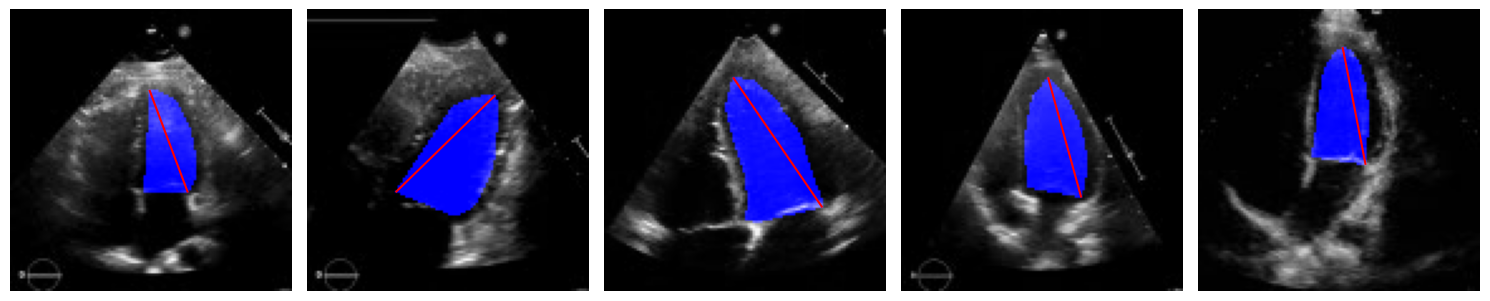
\includegraphics[width=0.9\linewidth]{orientation-var.png}
    \caption{Orientation variability in A4C views.}
    \label{fig:samples}
\end{figure}

These per frame descriptors are then used to estimate volumes using the area–length (bullet) method,

\begin{equation}
V_t = \frac{5}{6} \cdot |\Omega_t| \cdot L_t \cdot s^3, \quad s \in \mathbb{R}^+
\end{equation}

\noindent
where s is the pixel spacing in millimeters. Maximum and minimum values are identified as end-diastolic and end-systolic volumes, respectively. The heuristic ejection fraction is then computed as,

\begin{equation}
\widehat{\mathbf{EF}} = \left( \frac{\mathbf{V}_{\text{max}} - \mathbf{V}_{\text{min}}}{\mathbf{V}_{\text{max}}} \right) \times 100
\end{equation}

\subsection{Learning-Based Correction of Signed Error}

Although this heuristic method is a clinically established approach for estimating EF, its accuracy inherently depends on the fidelity of the segmentation and geometric assumptions can introduce systematic bias, particularly in irregular heart morphologies (see Fig.\ref{fig:segmentation-sequence}). To quantify and mitigate these deviations, some studies include a correction mechanism to identify segmentation outliers, and reduce their influence in EF estimate\cite{zhang2024automated}.

\begin{figure}
    \centering
    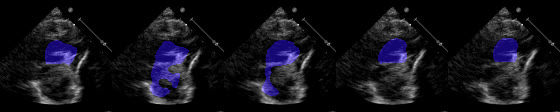
\includegraphics[width=0.9\linewidth]{segmentation_outlier.png}
    \caption{Segmentation outlier sequence exhibiting temporal inconsistency.}
    \label{fig:segmentation-sequence}
\end{figure}

This study introduces a learned correction strategy that predicts the signed error between the ground truth EF and the initial estimate $\widehat{EF}$, defined as:

\begin{equation}
    \varepsilon\ ={EF}_{true}\ -\ \widehat{\ EF}
\end{equation}

$\varepsilon$ was modeled using a set of interpretable descriptors extracted from the segmentation process, with the goal of characterizing the LV dynamic behavior. Among these, three were identified as the most effective predictors: the length ratio (minimum-to-maximum ventricular length), representing the extent of longitudinal contraction—a well-established marker of systolic function; the volume ratio (minimum-to-maximum ventricular volume), representing the heart’s pumping efficiency by approximating stroke volume normalized by chamber size; and the standard deviation (std) of the Dice similarity coefficient between consecutive segmentation masks, representing the temporal stability of the ResNet50-encoded U-Net predictions. The strength of association between each feature and the signed error is summarized in Table~\ref{tab:correlation-features}.

\begin{table}[ht]
\centering
\caption{Pearson and Spearman coefficients between features and $\varepsilon$.}
\label{tab:correlation-features}
\begin{tabular}{|l|c|c|}
\hline
\textbf{Feature}              & \textbf{Pearson} & \textbf{Spearman} \\
\hline
Length ratio                 & 0.417            & 0.408             \\
Volume ratio                 & 0.324            & 0.444             \\
Dice similarity std          & 0.310            & 0.219             \\
\hline
\end{tabular}
\end{table}


The strong linear correlation ($\tau_p = 0.892$) between volume and length ratios reflects their expected geometric coupling. However, combining both into a joint descriptor did not improve performance, nor did removing either of the two individually. These features illustrate that the heuristic method tends to slightly underestimate in cases where the ventricle contracts as expected, and overestimate in cases of reduced motion or abnormal contraction (see Fig.~\ref{fig:vr-lr}).

\begin{figure}
    \centering
    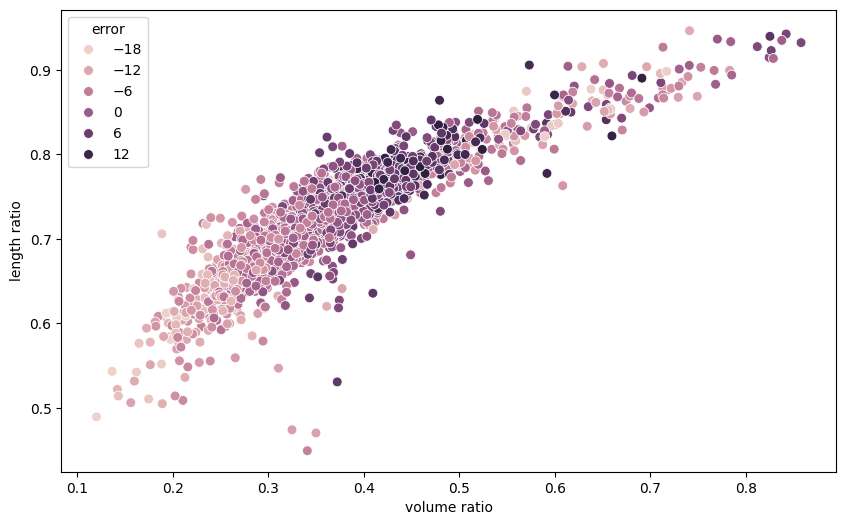
\includegraphics[width=0.6\linewidth]{volume_vs_length.png}
    \caption{Relationship between volume ratio and length ratio, with point color indicating the signed error $\varepsilon$.}
    \label{fig:vr-lr}
\end{figure}

Experiments were conducted using the scikit-learn implementations \cite{pedregosa2011scikit} of three regression models: Random Forest, K-Nearest Neighbors, and Gradient Boosting. Among these, the best overall performance on the validation set was achieved by Gradient Boosting, with the highest $R^2$ score and the lowest MAE and mean squared error (MSE), as shown in Table~\ref{tab:model_performance}. Consequently, this model was selected for hyperparameter tuning. The best-performing configuration was defined by a learning rate of 0.01, a maximum tree depth of 4, and 200 estimators.

\begin{table}[ht]
\centering
\caption{Performance comparison of candidate models on validation set}
\label{tab:model_performance}
\begin{tabular}{|l|c|c|c|}
\hline
\textbf{Model}           & \textbf{MAE} & \textbf{MSE} & \textbf{$R^{2}$} \\
\hline
Gradient Boosting       & 3.911048     & 26.991312    & 0.261009 \\
Random Forest           & 4.052565     & 27.856274    & 0.237327 \\
K-Nearest Neighbors     & 4.248252     & 30.141946    & 0.174748 \\
\hline
\end{tabular}
\end{table}

The regression model outputs $\hat{\varepsilon}$ are added to the initial EF estimates, representing a learned correction to the heuristic predictions based on segmentation and geometry. 

\section{Results}

The initial EF estimates on the test set yielded a MAE of 6.42\%, highlighting the limitations of segmentation and heuristic volume estimation under varying cardiac anatomies. After the learned correction term $\hat{\varepsilon}$ was added, the MAE was reduced to 4.69\%. 

\subsection{Residual Analysis and Statistical Testing}

The agreement between predicted and true EFs was further evaluated using Bland–Altman plots before and after the regression-based correction (see Fig. \ref{fig:bland-altman}). The original heuristic estimates exhibited a mean bias of $-2.50\%$ indicating systematic overestimation, with wide limits of agreement (LoA) ranging from $-18.08\%$ to $13.07\%$. After applying the Gradient Boosting correction, the mean bias was effectively reduced to $-0.22\%$ and LoA narrowed to $-12.72\%$ to $12.28\%$. This correction also led to a tighter clustering of errors around the zero-bias line and fewer outliers beyond LoA, suggesting improved consistency and clinical reliability of the final EF predictions.

To determine whether the observed improvement was statistically significant, additional analyses were performed on the absolute prediction errors. The distribution of the error reduction—defined as the difference between the heuristic and corrected absolute errors—was first evaluated for normality using the Kolmogorov-Smirnov (Lilliefors) test. A statistic value of $D=0.1529$ with $p=0.001$ was obtained, indicating a significant deviation from normality. 

\begin{figure}
    \centering
    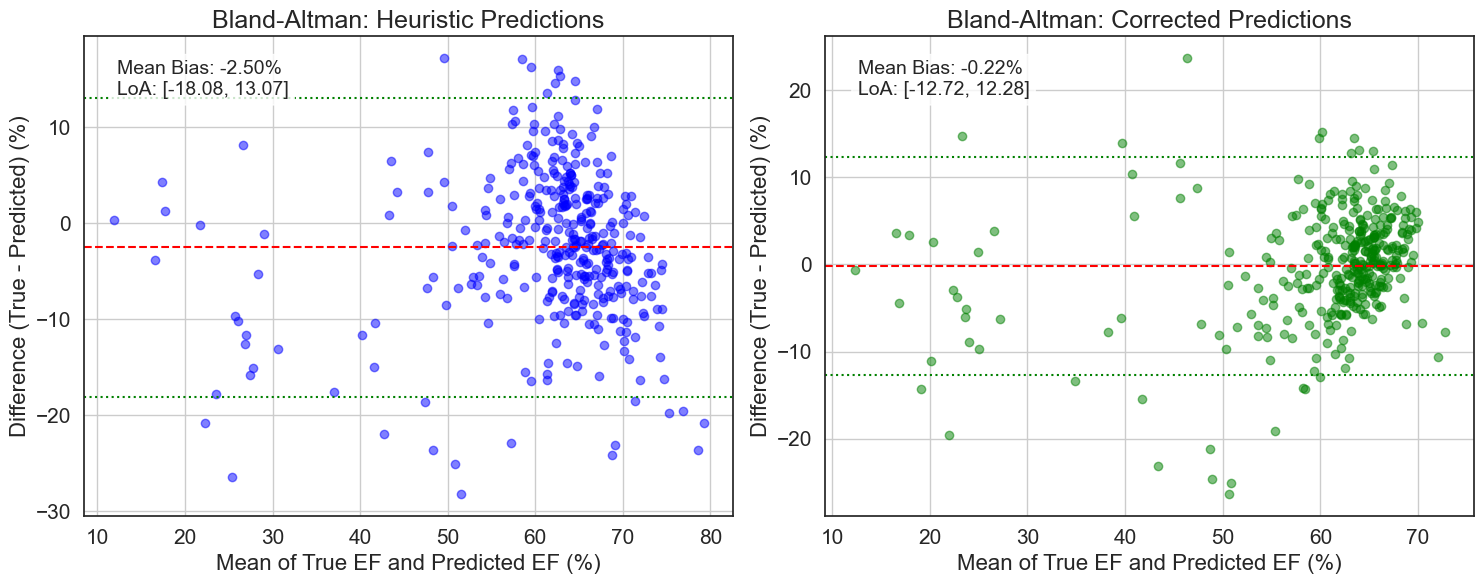
\includegraphics[width=1\linewidth]{bland-altman.png}
    \caption{Bland–Altman plots showing residuals before and after applying the learned correction term $\hat{\varepsilon}$.}
    \label{fig:bland-altman}
\end{figure}

Given the non-normal distribution of error differences, the Wilcoxon signed-rank test was applied. This test strongly rejected the null hypothesis of no improvement with $p < 10^{-6}$, confirming that the regression correction significantly reduced prediction error.

A more precise quantification of the improvement was obtained by using a nonparametric bootstrap (10000 iterations) to construct a 95\% confidence interval for the mean reduction in absolute error. The resulting interval ranged from 1.38\% to 2.10\%, with a midpoint of 1.74\%. As this interval lies entirely above zero, it provides strong evidence of systematic improvement across the test set.

\subsection{Interpretability and Feature Contribution}

The interpretability of the proposed pipeline is grounded in the integration of clearly defined geometric descriptors that are clinically relevant, enabling medical professionals to validate and understand the corrections applied to EF estimates. This hybrid approach aligns with prior works that combine convolutional networks with statistical models to refine the accuracy of ventricular volume measurements\cite{zhang2024automated}, or employ anatomical parameters as explanatory variables in cardiac segmentation\cite{wu2021automated}. Unlike black-box architectures based on 3D-CNN or Transformers—which prioritize algorithmic performance over transparency—the method presented here leverages interpretable geometric features (ventricular length and volume ratios) to ensure a direct correlation with clinical principles.

Feature relevance analysis using the SHAP (SHapley Additive exPlanations) method\cite{lundberg2017} (see Fig.\ref{fig:shap}) confirms the consistency between geometric predictors and corrected EF estimation errors. On the test set, volume ratio emerges as the most influential descriptor for predicting the error, followed by length ratio and Dice similarity standard deviation. These results validate the hypothesis that deviations in computed EF are predominantly driven by inconsistencies in volumetric dynamics throughout the cardiac cycle.

\begin{figure}
    \centering
    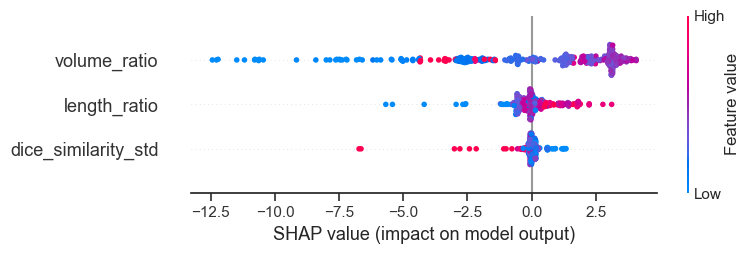
\includegraphics[width=0.7\linewidth]{shap_values.png}
    \caption{Features impact in regression-based correction.}
    \label{fig:shap}
\end{figure}

\subsection{Comparison with State of the Art Methodologies}

A comprehensive evaluation of left ventricular ejection fraction estimation models requires a detailed comparison with existing state-of-the-art methods. Table \ref{tab:comparison_models} presents such a comparative summary.
% Requires: \usepackage{array}
\begin{table}[h]
    \centering
    \setlength{\extrarowheight}{4pt}
    \caption{Comparison of EF estimation models by architecture, innovation, dataset, and performance.}
    \label{tab:comparison_models}
    \begin{tabular}{|>{\raggedright\arraybackslash}m{3cm}|>{\raggedright\arraybackslash}m{3cm}|>{\raggedright\arraybackslash}m{3cm}|>{\raggedright\arraybackslash}m{2.5cm}|}
        \hline
        \textbf{Architecture} & \textbf{Key Innovation} & \textbf{Dataset} & \textbf{MAE} \\ \hline
        ResNet50-encoded 2D U-Net + Area-Length + Regression (current methodology) & Interpretable pipeline correcting biases from segmentation and heuristic volume estimation. & EchoNet-Pediatric (A4C subset) & 4.69\% \\ \hline
        3D Convolutional Neural Network (3D CNN)\cite{echonetpediatric2023} & First AI model solely on a large, diverse pediatric dataset. & EchoNet-Pediatric & 3.66\% \\ \hline
        Quasi-Period Network (Parameterized Helix Trajectory + Neural CDE) + Variance Minimization\cite{qpart2025} & TTT framework for pediatric EF using quasi-periodic dynamics with guaranteed variance minimization & EchoNet-Dynamic \& EchoNet-Pediatric (stratified into Pre-School, School-Age, Adolescence, Adult cohorts) & Pre-School: 7.235\%, School Age: 6.706\%, Adolescence: 6.980\% \\ \hline
        DeepLabv3 (seg) + R(2+1)D (EF)\cite{ouyang2020echonet} & Spatiotemporal 3D CNN for video. & EchoNet-Dynamic & 4.1\% \\ \hline
        Hybrid CNN-Transformer (3D ResNet + RTM)\cite{efnet2025} & Residual Transformer Module for spatiotemporal analysis. & EchoNet-Dynamic & 3.7\% \\ \hline
    \end{tabular}
\end{table}

A critical distinction among the evaluated models lies in their foundational datasets: the EchoNet-Pediatric and EchoNet-Dynamic collections. While both datasets are derived from echocardiographic imaging, they differ in their target populations, data acquisition protocols, and labeling practices, reflecting distinct clinical priorities. For instance, EchoNet-Pediatric emphasizes age-specific cardiac measurements and pathology annotation relevant to children, whereas EchoNet-Dynamic was curated primarily for assessing ventricular function in adults.

The proposed pipeline was also evaluated on the EchoNet-Dynamic test set, achieving an initial MAE of 8.94\%, and after applying the learned correction, this metric was reduced to 7.34\%. While this result does not match state-of-the-art performance levels, it is important to acknowledge that analyzing pediatric echocardiography data presents unique challenges, which in turn affect model generalizability and clinical applicability. Pediatric patients have distinct anatomical and physiological characteristics, such as smaller cardiac structures and ongoing growth, necessitating age-specific normative values and measurement techniques. Additionally, the patterns and types of cardiac diseases encountered in this population differ substantially from those in adults Therefore, models trained exclusively on one population may not accurately capture the specific features of the other. Direct numerical comparisons between such models should be approached with caution, as they are grounded in separate clinical contexts.

Beyond population-specific considerations, computational demands influence clinical utility. While models employing 3D CNNs with transformer or spatiotemporal architectures achieve lower numerical error, their reliance on volumetric data demand significantly greater memory and processing power for both training and inference, leading to practical limitations in clinical environments. By contrast, clinical interpretability is prioritized in our approach through the use of a simpler architecture. Transparent intermediate outputs, such as visual tracings of cardiac structures, are provided by its segmentation-based methodology, aligning directly with established echocardiographic practices. In addition, explainability techniques are incorporated, and this clarity enhances clinician confidence and enables more informed diagnostic decisions. Such qualities are especially important in medical AI, as they facilitate validation by clinical experts, encourage responsible deployment, and support alignment with established diagnostic standards.

\section{Conclusions}



By combining a reliable heuristic approach with data-based corrections,  improved accuracy is achieved while keeping the process understandable for clinicians. Building on the well-known area-length method ensures that the pipeline remains connected to physiological principles, addressing the common issue of limited transparency in many deep learning models.

The addition of geometric descriptors helps capture the heart’s complex movements, reducing errors that frequently affect traditional methods. Reliable performance was confirmed through statistical and clinical evaluations, while explainability analyses verified that key features closely correspond  to medical relevance.

These results emphasize the potential of hybrid approaches that balance clinical interpretability with improved precision. Such solutions not only fit naturally into existing workflows but also have the capacity to make automated cardiac function assessment more accessible and widely adopted across different healthcare settings.



%
% ---- Bibliography ----
%
% BibTeX users should specify bibliography style 'splncs04'.
% References will then be sorted and formatted in the correct style.
%
% \bibliographystyle{splncs04}
% \bibliography{mybibliography}
%

\begin{thebibliography}{99}

\bibitem{azarmehr2020automated}
Azarmehr, N., Ye, X., Janan, F., Howard, J.P., Francis, D.P., Zolgharni, M.: Automated Segmentation of Left Ventricle in 2D echocardiography using deep learning. arXiv preprint arXiv:2003.07628 (2020). \doi{10.48550/arXiv.2003.07628}

\bibitem{moradi2019mfp}
Moradi, S., Ghelich Oghli, M., Alizadehasl, A., Shiri, I., Oveisi, N., Oveisi, M., Maleki, M., Dhooge, J.: MFP-Unet: A novel deep learning based approach for left ventricle segmentation in echocardiography. Physica Medica \textbf{67}, 58--69 (2019). \doi{10.1016/j.ejmp.2019.10.001}


\bibitem{kumar2025enhancing}
Kumar, V., Sharma, N.M., Mahapatra, P.K., Dogra, N., Maurya, L., Ahmad, F., Dahiya, N., Panda, P.: Enhancing Left Ventricular Segmentation in Echocardiograms Through GAN-Based Synthetic Data Augmentation and MultiResUNet Architecture. Diagnostics \textbf{15}(6), 663 (2025). \doi{10.3390/diagnostics15060663}


\bibitem{irshad2023lightunet}
Irshad, M., Yasmin, M., Sharif, M.I., Rashid, M., Sharif, M.I., Kadry, S.: A Novel Light U-Net Model for Left Ventricle Segmentation Using MRI. Mathematics \textbf{11}(14), 3245 (2023). \doi{10.3390/math11143245}

\bibitem{xu2022resunet}
Xu, S., Lu, H., Cheng, S., Pei, C.: Left Ventricle Segmentation in Cardiac MR Images via an Improved ResUnet. International Journal of Biomedical Imaging \textbf{2022}, 8669305 (2022). \doi{10.1155/2022/8669305}

\bibitem{wu2021automated}
Wu, H., Lu, X., Lei, B., Wen, Z.: Automated left ventricular segmentation from cardiac magnetic resonance images via adversarial learning with multi-stage pose estimation network and co-discriminator. Medical Image Analysis \textbf{68}, 101891 (2021). \doi{10.1016/j.media.2020.101891}

\bibitem{shi2024study}
Shi, S., Alimu, P., Mahemut, P.: The Study of Echocardiography of Left Ventricle Segmentation Combining Transformer and Convolutional Neural Networks. International Heart Journal \textbf{65}(5), 889--897 (2024). \doi{10.1536/ihj.23-638}

\bibitem{ouyang2020echonet}
Ouyang, D., He, B., Ghorbani, A., Yuan, N., Ebinger, J., Langlotz, C.P., Heidenreich, P.A., Harrington, R.A., Liang, D.H., Ashley, E.A., Zou, J.Y.: EchoNet-Dynamic: A Large New Cardiac Motion Video Data Resource for Medical Computer Vision. In: Medical Image Computing and Computer Assisted Intervention -- MICCAI 2020, Lecture Notes in Computer Science \textbf{12264}, 66--75 (2020). \doi{10.1007/978-3-030-59719-1_7}

\bibitem{Ali2025}
Ali, W., Alsabban, W., Shahbaz, M., Al-Laith, A., Almogadwy, B.: EFNet: estimation of left ventricular ejection fraction from cardiac ultrasound videos using deep learning. \textit{PeerJ Computer Science} \textbf{11}, e2506 (2025). \doi{10.7717/peerj-cs.2506}

\bibitem{Lang2015}
Lang, R.M., Badano, L.P., Mor-Avi, V., Afilalo, J., Armstrong, A., Ernande, L., Flachskampf, F.A., Foster, E., Goldstein, S.A., Kuznetsova, T., Lancellotti, P., Muraru, D., Picard, M.H., Rietzschel, E.R., Rudski, L., Spencer, K.T., Tsang, W., Voigt, J.-U.: Recommendations for cardiac chamber quantification by echocardiography in adults: An update from the American Society of Echocardiography and the European Association of Cardiovascular Imaging. \textit{European Heart Journal - Cardiovascular Imaging} \textbf{16}(3), 233--271 (2015). \doi{10.1093/ehjci/jev014}

\bibitem{echonetpediatric2023}
Reddy, C.D., Lopez, L., Ouyang, D., Zou, J.Y., He, B.: EchoNet-Pediatric: A Large Pediatric Echocardiography Video Data Resource for Medical Machine Learning. Stanford University (2023). \doi{10.71718/d05h-gy43}

\bibitem{leclerc2019camus}
Leclerc, B., Smistad, O., Caballero, J., Frangié, P.A., Bernard, O., et al.: Automatic left ventricular myocardium delineation in echocardiographic images with deep learning: the CAMUS project. IEEE Transactions on Medical Imaging \textbf{38}(9), 2198--2210 (2019). \doi{10.1109/TMI.2019.2900516}

\bibitem{paszke2019pytorch}
Paszke, A., Gross, S., Massa, F., Lerer, A., Bradbury, J., Chanan, G., Killeen, T., Lin, Z., Gimelshein, N., Antiga, L., Desmaison, A., Kopf, A., Yang, E., DeVito, Z., Raison, M., Tejani, A., Chilamkurthy, S., Steiner, B., Fang, L., Bai, J., Chintala, S.: PyTorch: An Imperative Style, High-Performance Deep Learning Library. In: Advances in Neural Information Processing Systems 32 (NeurIPS 2019), 8024--8035 (2019). \url{https://pytorch.org}

\bibitem{qubvel2019smp}
Qubvel: Segmentation Models PyTorch. GitHub repository and documentation, 2019--2024. \url{https://github.com/qubvel/segmentation_models.pytorch} \url{https://segmentation-models-pytorch.readthedocs.io}

\bibitem{deng2009imagenet}
Deng, J., Dong, W., Socher, R., Li, L.J., Li, K., Fei-Fei, L.: ImageNet: A large-scale hierarchical image database. In: 2009 IEEE Conference on Computer Vision and Pattern Recognition (CVPR), pp. 248--255 (2009). \doi{10.1109/CVPR.2009.5206848}

\bibitem{akiba2019optuna}
Akiba, T., Sano, S., Yanase, T., Ohta, T., Koyama, M.: Optuna: A next-generation hyperparameter optimization framework. In: Proceedings of the 25th ACM SIGKDD International Conference on Knowledge Discovery \& Data Mining, pp. 2623--2631 (2019). \doi{10.1145/3292500.3330701}

\bibitem{zhang2024automated}
Zhang, Y., Liu, B., Bunting, K.V., Brind, D., Thorley, A., Karwath, A., Lu, W., Zhou, D., Wang, X., Mobley, A.R., Tica, O., Gkoutos, G.V., Kotecha, D., Duan, J.: Development of automated neural network prediction for echocardiographic left ventricular ejection fraction. Frontiers in Medicine \textbf{11}, 1354070 (2024). \doi{10.3389/fmed.2024.1354070}

\bibitem{pedregosa2011scikit}
Pedregosa, F., Varoquaux, G., Gramfort, A., Michel, V., Thirion, B., Grisel, O., Blondel, M., Prettenhofer, P., Weiss, R., Dubourg, V., Vanderplas, J., Passos, A., Cournapeau, D., Brucher, M., Perrot, M., Duchesnay, E.: Scikit-learn: Machine Learning in Python. Journal of Machine Learning Research \textbf{12}, 2825--2830 (2011). \url{https://scikit-learn.org}

\bibitem{lundberg2017}
Lundberg, S.M., Lee, S.I.: A unified approach to interpreting model predictions. In: \textit{Advances in Neural Information Processing Systems}, \textbf{30} (2017)

\bibitem{qpart2025}
Liu, J., Qin, T., Liu, H., Shi, Y., Mou, L., Zhu, X.X., Wang, S., Li, H.: Q-PART: Quasi-Periodic Adaptive Regression with Test-time Training for Pediatric Left Ventricular Ejection Fraction Regression. In: \textit{Proceedings of the IEEE/CVF Conference on Computer Vision and Pattern Recognition (CVPR)} (2025). \url{https://doi.org/10.48550/arXiv.2503.04131}

\bibitem{efnet2025}
Ali, W., Alsabban, W., Shahbaz, M., Al-Laith, A., Almogadwy, B.: EFNet: Estimation of left ventricular ejection fraction from cardiac ultrasound videos using deep learning. \textit{PeerJ Comput. Sci.} \textbf{11}, e2506 (2025). \url{https://doi.org/10.7717/peerj-cs.2506}

\end{thebibliography}
\end{document}